Interpolacija je postupak kojim od zadanih točaka neke funkcije $f(x)$ dolazimo
do funkcije $g(x)$ koja prolazi tim točkama i \textit{blisko prati} $f(x)$.

Interpolacija uključuje pogreške mjerenja tako da je netočno reći $g(x) = f(x)$,
no polinom ili po dijelovima funkcija koju dobijemo interpolacijom će dati
dobar uvid u međuvrijednosti zadanih točaka.

\begin{center}
    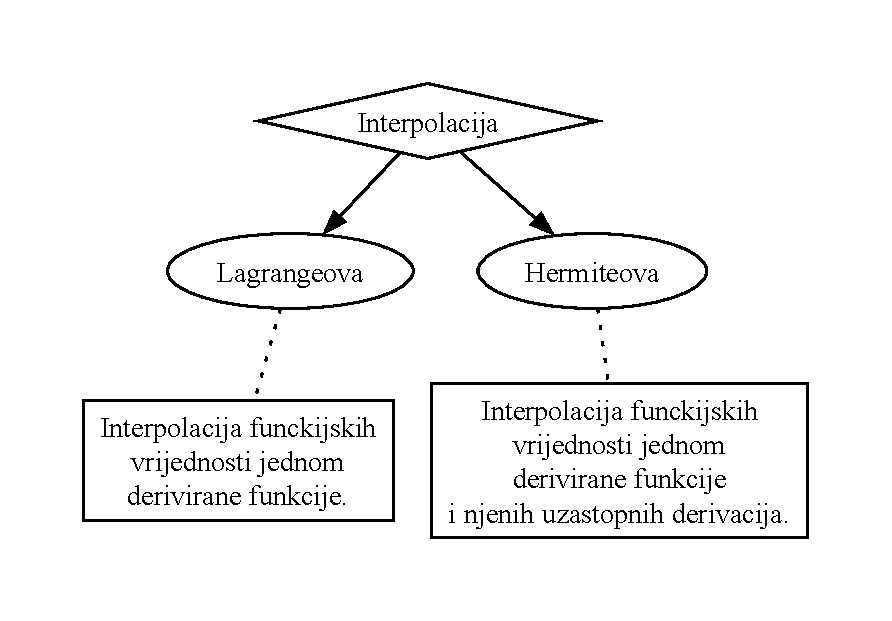
\includegraphics[width=0.5\linewidth]{interpolation.pdf}
\end{center}

\begin{theorem}[egzistencija i jedinstvenost polinoma]
    Neka je $n\in\mathbb{N}_0$. Za zadane točke $(x_k,y_k)$, gdje je $y_k\coloneq f(x_k), k\in[0,n]$ i $x_i\neq x_j$ za $i\neq j$ postoji jedinstveni interpolacijski polinom najviše stupnja $n$

    $$
        p_n(x)=a_0+a_1x+\dots+a_nx^n
    $$

    za kojeg vrijedi

    $$
        p_n(x_k) = y_k,\qquad k\in[0,n]
    $$
\end{theorem}

\textbf{Dokaz:}

\bigskip

Neka je polinom $p_n(x)=a_0+a_1x+a_2x^2+\dots+a_nx^n$ polinom stupnja najviše $n$.

Uvjete interpolacije zapisujemo u obliku

\begin{gather*}
    p_n(x_0)=a_0+a_1x_0+a_2x_0^2+\dots+a_nx_0^n=y_0\\
    p_n(x_1)=a_0+a_1x_1+a_2x_1^2+\dots+a_nx_1^n=y_1\\
    \vdots\\
    p_n(x_n)=a_0+a_1x_n+a_2x_n^2+\dots+a_nx_n^n=y_2
\end{gather*}

Dobiven je sustav od $n+1$ linearne jednadžbe s $n+1$ nepoznanicom (koeficijenti $a_i, i\in[0,n]$ su nepoznanice).

Pitamo se ima li navedeni sustav rješenje i je li ono \textbf{jedinstveno}.
Za to je dovoljno provjeriti je li odgovarajuća matrica sustava regularna.\footnote{Matrica sustava je regularna ako joj je determinanta različita od 0.}
Matrični sustav koji promatramo je

\begin{equation}
    \label{unique_poly}
    \begin{bmatrix}
        1&x_0&x_0^2&\cdots&x_0^n\\
        1&x_1&x_1^2&\cdots&x_1^n\\
        \vdots\vdots&\vdots&\vdots&\vdots\\
        1&x_n&x_n^2&\cdots&x_n^n\\
    \end{bmatrix}
    \cdot
    \begin{bmatrix}
        a_0\\
        a_1\\
        \vdots\\
        a_n
    \end{bmatrix}
    =
    \begin{bmatrix}
        y_0\\
        y_1\\
        \vdots\\
        y_n
    \end{bmatrix}
\end{equation}

Želimo odrediti $D_n$, gdje je

$$
D_n = \begin{vmatrix}
    1&x_0&x_0^2&\cdots&x_0^n\\
    1&x_1&x_1^2&\cdots&x_1^n\\
    \vdots&\vdots&\vdots&\vdots&\vdots\\
    1&x_n&x_n^2&\cdots&x_n^n\\
\end{vmatrix}
$$

\newpage

Vandermondeova determinanta $D_n$ je poznata.
Ako je $D_n \neq 0$, tada sustav \ref{unique_poly} ima jedinstveno rješenje.
Definiramo pomoćnu determinantu oblika

$$
V_n(x) = \begin{vmatrix}
    1&x_0&x_0^2&\cdots&x_0^n\\
    1&x_1&x_1^2&\cdots&x_1^n\\
    \vdots&\vdots&\vdots&\vdots&\vdots\\
    1&x&x^2&\cdots&x^n\\
\end{vmatrix},
\qquad V_n(x_n) = D_n
$$

Promatramo li $V_n(x)$ kao funkciju od $x$, razvojem po posljednjem retku uočavamo da je $V_n(x)$
polinom stupnja najviše $n$ u varijabli $x$, a vodeći koeficijent tog polinoma je determinanta $D_{n-1}$.
Zaista vrijedi

\begin{gather*}
V_n(x)=(-1)^{n+1}\cdot\begin{vmatrix}
    x_0&x_0^2&\cdots&x_0^n\\
    x_1&x_1^2&\cdots&x_1^n\\
    \vdots&\vdots&\vdots&\vdots\\
    x_{n-1}&x_{n-1}^2&\cdots&x_{n-1}^n\\
\end{vmatrix}\cdot1
+(-1)^{n+2}\cdot\begin{vmatrix}
    1&x_0^2&\cdots&x_0^n\\
    1&x_1^2&\cdots&x_1^n\\
    \vdots&\vdots&\vdots&\vdots\\
    1&x_{n-1}^2&\cdots&x_{n-1}^n\\
\end{vmatrix}\cdot x
+\cdots\\
+\underbrace{(-1)^{2n}\cdot\begin{vmatrix}
    1&x_0&\cdots&x_0^{n-1}\\
    1&x_1&\cdots&x_1^{n-1}\\
    \vdots&\vdots&\vdots&\vdots\\
    1&x_{n-1}&\cdots&x_{n-1}^{n-1}\\
\end{vmatrix}}_{D_{n-1}}\cdot x^n
\end{gather*}

Dakle, vodeći koeficijent (koeficijent uz $x^n$) je

\begin{equation}
\label{unique_poly_coeff}
D_{n-1} = (-1)^{2n}\cdot\begin{vmatrix}
    1&x_0&\cdots&x_0^{n-1}\\
    1&x_1&\cdots&x_1^{n-1}\\
    \vdots&\vdots&\vdots&\vdots\\
    1&x_{n-1}&\cdots&x_{n-1}^{n-1}\\
\end{vmatrix}=\begin{vmatrix}
    1&x_0&\cdots&x_0^{n-1}\\
    1&x_1&\cdots&x_1^{n-1}\\
    \vdots&\vdots&\vdots&\vdots\\
    1&x_{n-1}&\cdots&x_{n-1}^{n-1}\\
\end{vmatrix}.
\end{equation}

Primijetimo da, ako se u $V_n(x)$ redom uvrste $x_0,x_1,\dots,x_{n-1}$, vrijedit će

$$
V_n(x_0)=V_n(x_1)=\dots=V_n(x_{n-1})=0,
$$

što povlači da su $x_0,x_1,\dots,x_{n-1}$ nultočke polinoma $V_n(x)$ koji je polinom $n$-tog stupnja.
Da bi polinom $n$-tog stupnja bio potpuno definiran, trebaju biti poznate nultočke i njegov
vodeći koeficijent (\ref{unique_poly_coeff}). Dakle, traženi polinom je

$$
V_n(x) = D_{n-1}(x-x_0)(x-x_1)\dots(x-x_{n-1}).
$$

Ako uvrstimo $x_n$ u $V_n(x)$, dobivamo rekurzivnu formulu za $D_n$, odnosno

$$
D_n=V_n(x_n)=D_{n-1}(x_n-x_0)(x_n-x_1)\dots(x_n-x_{n-1}).
$$

Trivijalno vrijedi $D_0 = 1$ te lako dobivamo

$$
D_n = \prod_{0\leq j<i\leq n}(x_i-x_j).
$$

Budući da je $x_i\neq x_j$ za $i\neq j$, onda je $D_n\neq 0$, a vrijedi i obrat.
Dakle, matrica sustava je regularna (jer $D_n\neq 0$) i stoga postoji jedinstveno rješenje
$(a_0,a_1,\dots,a_n)$ što povlači da postoji jedinstveni interpolacijski polinom.
